\documentclass[11pt]{article}
 
\usepackage[margin=1in]{geometry}
\usepackage{amsmath,amsthm,amssymb}
\usepackage{graphics}
\usepackage{graphicx}
\usepackage{subcaption}
\usepackage{hyperref}
\usepackage{changepage}

\usepackage{listings}
\usepackage{color}

\definecolor{dkgreen}{rgb}{0,0.6,0}
\definecolor{gray}{rgb}{0.5,0.5,0.5}
\definecolor{mauve}{rgb}{0.58,0,0.82}
\lstset{frame=tb,
  language=Python,
  aboveskip=3mm,
  belowskip=3mm,
  showstringspaces=false,
  columns=flexible,
  basicstyle={\small\ttfamily},
  numbers=none,
  numberstyle=\tiny\color{gray},
  keywordstyle=\color{blue},
  commentstyle=\color{dkgreen},
  stringstyle=\color{mauve},
  breaklines=true,
  breakatwhitespace=true,
  tabsize=3
}

\def\infinity{\rotatebox{90}{8}}
 
\newcommand{\N}{\mathbb{N}}
\newcommand{\R}{\mathbb{R}}
\newcommand{\Z}{\mathbb{Z}}
\newcommand{\Q}{\mathbb{Q}}
 
\newenvironment{theorem}[2][Theorem]{\begin{trivlist}
\item[\hskip \labelsep {\bfseries #1}\hskip \labelsep {\bfseries #2.}]}{\end{trivlist}}
\newenvironment{lemma}[2][Lemma]{\begin{trivlist}
\item[\hskip \labelsep {\bfseries #1}\hskip \labelsep {\bfseries #2.}]}{\end{trivlist}}
\newenvironment{exercise}[2][Exercise]{\begin{trivlist}
\item[\hskip \labelsep {\bfseries #1}\hskip \labelsep {\bfseries #2.}]}{\end{trivlist}}
\newenvironment{problem}[2][Problem]{\begin{trivlist}
\item[\hskip \labelsep {\bfseries #1}\hskip \labelsep {\bfseries #2.}]}{\end{trivlist}}
\newenvironment{question}[2][Question]{\begin{trivlist}
\item[\hskip \labelsep {\bfseries #1}\hskip \labelsep {\bfseries #2.}]}{\end{trivlist}}
\newenvironment{corollary}[2][Corollary]{\begin{trivlist}
\item[\hskip \labelsep {\bfseries #1}\hskip \labelsep {\bfseries #2.}]}{\end{trivlist}}
 
\begin{document}
 
\title{CS281A - Problem Set 2}
\author{Andrea Bajcsy}
 
\maketitle
 
\begin{problem}{2.1}
\text{ }\\

(a) We can formulate the polynomial regression problem as a form of linear prediction by soliving the general linear model equation $X\alpha = y$ where:
\\
\[
X=
  \begin{bmatrix}
    1 & t_{1} & t^2_{1} & ... & t^D_{1}\\
    1 & t_{2} & t^2_{2} & ... & t^D_{2}\\
    1 & t_{3} & t^2_{3} & ... & t^D_{3}\\
    ...\\
    1 & t_{n} & t^2_{n} & ... & t^D_{n}\\
  \end{bmatrix}
\alpha=
	\begin{bmatrix}
		\alpha_{1}\\
		\alpha_{2}\\
		\alpha_{3}\\
		...\\
		\alpha_{D}\\
	 \end{bmatrix}
y=
	\begin{bmatrix}
		y_{1}\\
		y_{2}\\
		y_{3}\\
		...\\
		y_{n}\\
	 \end{bmatrix}
\]

(b) Figure \ref{fig:2b} shows a plot of the mean-squared error R(D) vs. Degree $D \in {1,2,...n-1}$ when using the data in y.dat and t.dat. See back for code that performs least-squares fit of a polynomial of degree D. 
\begin{figure}[h!]
  \centering
  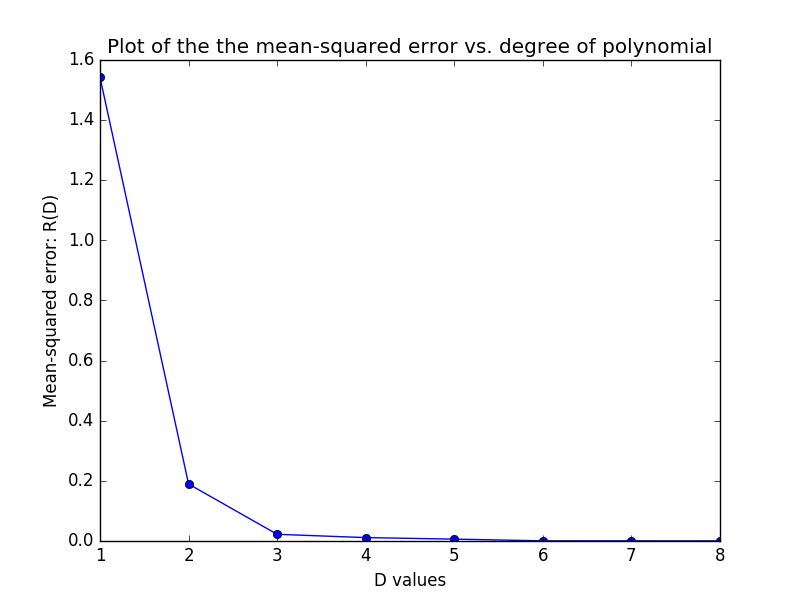
\includegraphics[scale=0.5]{figs/2b.png}
  \caption{D vs. R(D)}
  \label{fig:2b}
\end{figure}

(c) 
With the degree n-1 fit, we get (approximately) zero mean-squared error since the function fits exactly to every data point. What happens if you try to fit a polynomial of degree n? Why? To fit a polynomial of degree n, we will be solving $X\alpha = y$, where $X^{n~x~n}$.
\[
	\begin{bmatrix}
	1 & t_{1} & t^2_{1} & ... & t^n_{1}\\
	1 & t_{2} & t^2_{2} & ... & t^n_{2}\\
	1 & t_{3} & t^2_{3} & ... & t^n_{3}\\
	...\\
	1 & t_{n} & t^2_{n} & ... & t^n_{n}\\
	\end{bmatrix}
	\begin{bmatrix}
		\alpha_{1}\\
		\alpha_{2}\\
		\alpha_{3}\\
		...\\
		\alpha_{n}\\
	 \end{bmatrix}
=
	\begin{bmatrix}
		y_{1}\\
		y_{2}\\
		y_{3}\\
		...\\
		y_{n}\\
	 \end{bmatrix}
\]
Using ordinary least-squares, we solve for $\alpha$ = $(X^{T}X)^{-1}X^{T}y$. We see there are more columns than rows, so the matrix $X^{T}X$ will not be invertible and the solution is not defined. 

(d) Figure \ref{fig:2d} shows a plot of the degree $D \in {1,2,...n-1}$ versus the mean-squared error R(D) and $\tilde{R}$ when using the data in y.dat, yfresh.dat, and t.dat. Even though we are fitting D = n-1 degree polynomial to the new yfresh.dat data, the model was trained on y.dat and will approximate yfresh.dat with greater error than the data it was trained on and cannot be a perfect estimator. Thus, the error appears to plateu for the same values of D with yfresh.dat or y.dat but at a higher error value when using yfresh.dat. Choose the minimal degree D after which the error doesn't change within some small $\epsilon$ bound. This ensures that you will not be overfitting. 
\begin{figure}[h!]
  \centering
  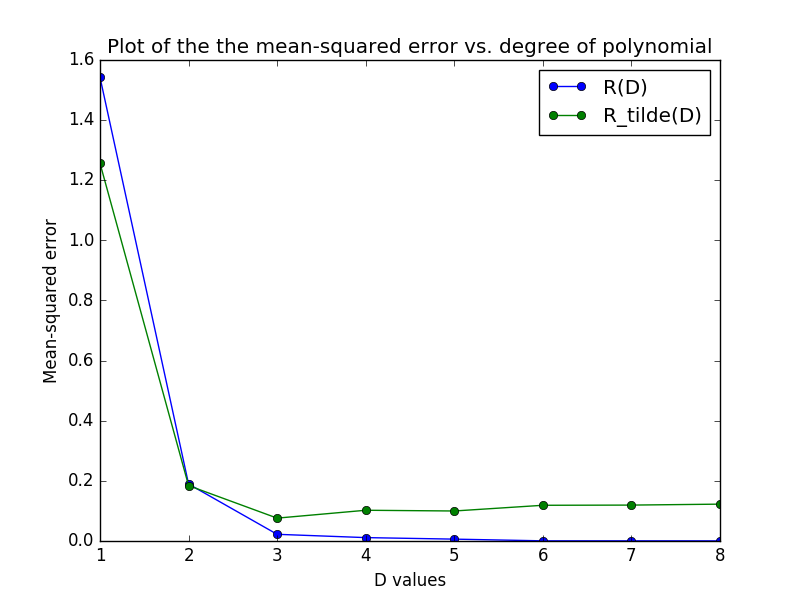
\includegraphics[scale=0.5]{figs/2d.png}
  \caption{D vs. R(D) and $\tilde{R}$}
  \label{fig:2d}
\end{figure}

(e) Figure \ref{fig:2e} shows a plot of the degree $D \in {2,...9}$ versus the mean-squared error $\tilde{R}$ and F(D) when using the data in y.dat, yfresh.dat, and t.dat. The minimizing arguments of the two functions related in that F(D) adds an extra cost on the number of degrees you are using. Since the lowest error for R(D) and $\tilde(R(D))$ functions when D=3, so we see a penalization of greater D's. 
\begin{figure}[h!]
  \centering
  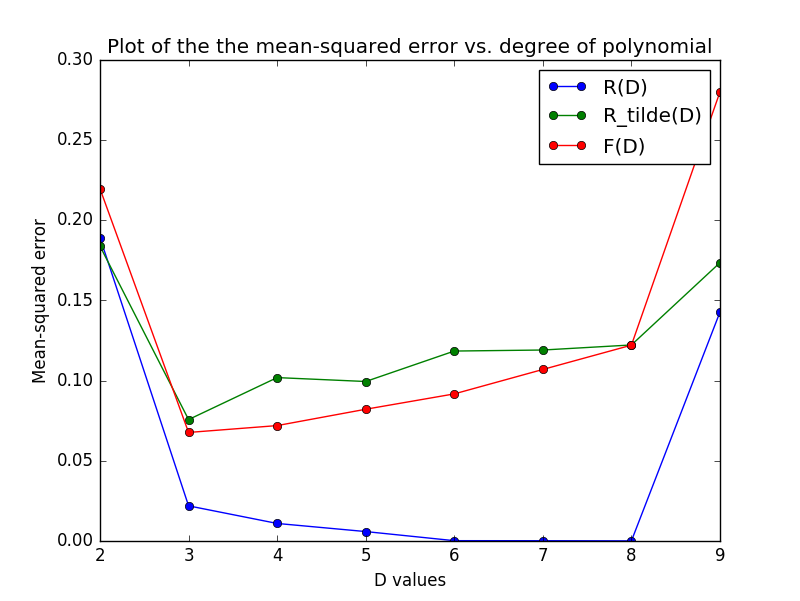
\includegraphics[scale=0.5]{figs/2e_2.png}
  \caption{D vs. $\tilde{R}$ and F(D)}
  \label{fig:2e}
\end{figure}

\end{problem}
 
\begin{problem}{2.2}
\text{ }\\

(a) Prove that A is a convex function.
\begin{proof}
By definition, 
\[ A(\eta) = log(\int_\gamma h(y)e^{\eta y}\,dy )~~,~~p_{\eta}(y) = h(y)e^{\eta y-A(\eta)} \]
To prove convexity, we want to take the second derivative. Let:
\[B(\eta) = \int_\gamma h(y)e^{\eta y}\,dy \]
Then the first derivative we get:
\[ \frac{\partial A(\eta)}{\partial \eta}
   = \left( \frac{1}{B(\eta)}\right)
     \left(\frac{\partial B(\eta)}{\partial \eta}\right) 
   = \frac{\int_\gamma h(y)e^{\eta y} y \,dy}{\int_\gamma h(y)e^{\eta y}\,dy}
   = \frac{\int_\gamma h(y)e^{\eta y - A(\eta)} y \,dy}{\int_\gamma h(y)e^{\eta y - A(\eta)}\,dy}
   =E_{p_{\eta}}[y]\]
Taking the second derivative we have:
\[ \frac{\partial}{\partial \eta}~\frac{B'(\eta)}{B(\eta)}
   = \frac{\partial}{\partial \eta}\left( B'(\eta)\frac{1}{B(\eta)}\right)
   = \frac{B''(\eta)}{B(\eta)} - \frac{(B'(\eta))^2}{B(\eta)^2}\]
\[= \frac{\int_\gamma h(y)e^{\eta y} y^2 \,dy}{\int_\gamma h(y)e^{\eta y}\,dy}~-~(E_{p_{\eta}}[y])^2
   = \frac{\int_\gamma h(y)e^{\eta y - A(\eta)} y \,dy}{\int_\gamma h(y)e^{\eta y - A(\eta)}\,dy}~-~(E_{p_{\eta}}[y])^2\]
\[ = E_{p_{\eta}}[y^2]~-~(E_{p_{\eta}}[y])^2 
   = Var_{p_{\eta}}[y] ~\succeq~0 \]

Since $Var_{p_{\eta}}$ is positive definite, we have shown that $A(\eta)$ is convex.
\end{proof}

(b) Express KL divergance in terms of $A(\eta)$ and $A'(\eta)$. 

\[ D(p_{\eta} || p_{\eta}) = E_{\eta} \left(log(\frac{h(y)e^{\eta y - A(\eta)}}{h(y)e^{\tilde \eta y - A(\tilde \eta)}})\right)\]
\[= \int_y log \left(e^{(\eta - \tilde{n})y - (A(\eta) - A(\tilde{\eta}))} p_{\eta}(y) \right) \,dy \]
\[= \int_y \left((\eta - \tilde{n})y - (A(\eta) - A(\tilde{\eta})\right) h(y)e^{\eta y - A(\eta)} \,dy \]
\[= (\eta - \tilde{n})\int_y h(y)e^{\eta y - A(\eta)}y \,dy - (A(\eta) - A(\tilde{\eta})) \int_y h(y)e^{\eta y - A(\eta)} \,dy \]
\[= (\eta - \tilde{n})A' - A(\eta) + A(\tilde{\eta}) \]

Since $A\ = \int_y h(y)e^{\eta y - A(\eta)}y $ and $\int_y p_{\eta}(y)dy = 1 $ by definition.
\\

(i) Bernoulli random variable:
\\
\[p_{\eta}(y) = \eta^{y}(1-\eta)^{1-y}, y \in {0,1}, n \in (0,1)\]
\[ = e^{ylog(\eta) + (1-y)log(1-\eta)} = e^{ylog(\frac{\eta}{1-\eta}) - log(1+e^{\frac{\eta}{1-\eta}})}\]

\begin{adjustwidth}{2.5em}{0pt}
Thus, we have $A(\eta) = log(1+e^{\eta})$ and $A^{*}(t) = sup_{\eta\in R}~ \left\{\eta t - log(1+e^{\eta}\right\}$. We now take the gradient of $A^{*}$ with respect to $\eta$, set this to 0 in order to solve the optimization problem, and then solve for $\eta$ in terms of $t$.
\end{adjustwidth}

\[\nabla_{\eta} A^{*}(t) = t - \frac{e^{\eta}}{1+e^{\eta}} \]
\[0  = t - \frac{e^{\eta}}{1+e^{\eta}} \implies t = \frac{e^{\eta}}{1+e^{\eta}} \]
\[ \frac{1}{t} = \frac{1+e^{\eta}}{e^{\eta}} = \frac{1}{e^{\eta}} + 1 \implies \frac{1}{t} - 1 = \frac{1}{e^{\eta}}\]
\[e^{\eta} = \frac{1}{\frac{1}{t} - 1} \implies \eta = log(\frac{1}{\frac{1}{t} - 1})\]
\[\eta = -log(\frac{1}{t} - 1))\]

\begin{adjustwidth}{2.5em}{0pt}
Substituting this back into our equation, we get:
\end{adjustwidth}

\[A^{*}(t) = -tlog(\frac{1}{t}-1) - log(1+e^{-log(\frac{1}{t}-1)}) = -tlog(\frac{1}{t}-1) + log(1-t)\]
\[= tlog(t) - tlog(1-t) + log(1-t) = tlog(t) + (1-t)log(1-t)\]

(ii) Gaussian random variable (based on notes from class):
\\
\[p_{\eta}(y) = \frac{e^{\frac{-y^{2}}{2}}}{\sqrt{2\pi}}e^{yn - \frac{\eta^2}{2}}\]

\begin{adjustwidth}{2.5em}{0pt}
Thus, we have $A(\eta) = \frac{\eta^2}{2}$ and $A^{*}(t) = sup_{\eta\in R}~ \left\{\eta t - \frac{\eta^2}{2}\right\}$. 
\end{adjustwidth}

\[\nabla_{\eta} A^{*}(t) = t - n \]
\[0 = t - n \implies t = n \]

\begin{adjustwidth}{2.5em}{0pt}
Substituting this back into our equation, we get:
\end{adjustwidth}
\[A^{*}(t) = t^2 - \frac{t^2}{2} = \frac{t^2}{2}\]

(iii) Poisson random variable: 
\\
\[p_{\eta}(y) = \frac{1}{y!}e^{y\eta - e^{\eta}} \]

\begin{adjustwidth}{2.5em}{0pt}
Thus, we have $A(\eta) = e^{\eta}$ and $A^{*}(t) = sup_{\eta\in R}~ \left\{\eta t - e^{\eta}\right\}$. 
\end{adjustwidth}

\[\nabla_{\eta} A^{*}(t) = t - e^{\eta} \]
\[0 = t - e^{\eta} \implies log(t) = n \]

\begin{adjustwidth}{2.5em}{0pt}
Substituting this back into our equation, we get:
\end{adjustwidth}
\[A^{*}(t) = tlog(t) e^{log(t)} = tlog(t) - t = t(log(t) - 1)\]

(d) Prove that $A^{*}$ is always a convex function.
\begin{proof}
If $A^{*}$ is always a convex function, then it must satisfy the definition of convexity: 
\[A^{*}(\alpha t_{1} + (1-\alpha)t_{2}) \leq \alpha A^{*}(t_{1}) + (1-\alpha)A^{*}(t_{2})\]

We know that $A^{*}$ is defined by:
\[A^{*}(\alpha t_{1} + (1-\alpha)t_{2}) = sup_{\eta}\left\{{\eta(\alpha t_{1} + (1-\alpha)t_{2}) - A(\eta)}\right\}\]
\[= sup_{\eta}\left\{{\eta(\alpha t_{1} + (1-\alpha)t_{2}) - \alpha A(\eta) - (1-\alpha)A(\eta)}\right\}\]
\[= sup_{\eta}\left\{{\alpha(\eta t_{1} - A(\eta)) + (1-\alpha)(\eta t_{2}-A(\eta))}\right\}\]

Let $h(\eta) = \eta t_{1} - A(\eta)$ and $k(\eta) = \eta t_{2}-A(\eta)$. We know that: 
\[sup_{\eta}(h(\eta) + k(\eta)) \leq sup_{\eta}(h(\eta)) + sup_{\eta}(k(\eta))\]

By this property and after resubstituting, we have shown: 

\[A^{*}(\alpha t_{1} + (1-\alpha)t_{2}) \leq \alpha A^{*}(t_{1}) + (1-\alpha)A^{*}(t_{2})\]

And that $A^{*}$ is always a convex function. 

\end{proof}

\end{problem}

\begin{problem}{2.3}
\text{ }\\

(a) By definition, we have likelihood of $\eta$ as:

\[l(\eta; y_1,...y_n) = log(p(y_1,...,y_n|\eta)) = log(h(y_1,...y_n)) + \eta^T\sum^{n}_{i=1}y_i-nA(\eta)\]

\begin{adjustwidth}{2.5em}{0pt}
We differentiate and solve for $\hat{\eta}$ (assuming the inverse function exists under suitable regularity conditions):
\end{adjustwidth}

\[\frac{\partial}{\partial\eta}l(\eta; y_1,...y_n) = \sum^{n}_{i=1}y_i-n\frac{\partial}{\partial\eta}A(\eta)\]
\[\frac{\partial}{\partial\eta}A(\eta) = \frac{\sum^{n}_{i=1}y_i}{n} \implies \hat{\eta} = (A'^{-1})(\frac{\sum^{n}_{i=1}y_i}{n})\]

(b) Closed-form estimates for MLE in Poisson, Bernoulli, Gaussian models:
\\

Poisson
\[\frac{\partial}{\partial\eta}A(\eta) = e^{\eta} = \frac{\sum^{n}_{i=1}y_i}{n}\]
\[\hat{\eta} = log(\frac{\sum^{n}_{i=1}y_i}{n}) \]

Bernoulli (where $\frac{\sum^{n}_{i=1}y_i}{n} \neq 1$)
\[\frac{\partial}{\partial\eta}A(\eta) = \frac{e^{\eta}}{1+e^{\eta}} = \frac{\sum^{n}_{i=1}y_i}{n}\]
\[\hat{\eta} = log(\frac{\frac{\sum^{n}_{i=1}y_i}{n}}{1-\frac{\sum^{n}_{i=1}y_i}{n}})\]

Gaussian
\[\frac{\partial}{\partial\eta}A(\eta) = \eta = \frac{\sum^{n}_{i=1}y_i}{n} \]
\[\hat{\eta} = \frac{\sum^{n}_{i=1}y_i}{n}\]

(c)
\begin{adjustwidth}{2.5em}{0pt}
We know that $E(\bar{y}) = A'(\eta^{*})$ and by definition of MLE with respect to $\eta$, we have:
\end{adjustwidth}

\[max_{\eta}\left\{{\eta\sum^{n}_{i=1}{y_i}-nA(\eta)}\right\} = max_{\eta}\left\{{\eta\bar{y}-A(\eta)}\right\} = min_{\eta}\left\{{-\eta\bar{y}+A(\eta)}\right\}\]

\begin{adjustwidth}{2.5em}{0pt}
Thus, we know that as $n \rightarrow \infinity$, then $\bar{y} \rightarrow A'(\eta^{*})$. Additionally, we can add or subtract any terms to this equation that do not depend on $\eta$, since they are just constants. We can substitute this into the above equation to get:
\end{adjustwidth}

\[\hat{\eta} = min_{\eta}\left\{{-\eta A'(\eta^{*})+A(\eta)}\right\} = min_{\eta}\left\{{-\eta A'(\eta^{*})+A(\eta) + \eta^{*}A'(\eta^{*}) - A(\eta^{*})}\right\}\]

\begin{adjustwidth}{2.5em}{0pt}
After some rearranging of terms, we get the final equation:
\end{adjustwidth}

\[\hat{\eta}= min_{\eta}\left\{ A(\eta) - A(\eta^{*}) - A'(\eta^{*})(\eta - \eta^{*})\right\} \]

(d) 
\begin{adjustwidth}{2.5em}{0pt}
Assume A is strictly convex and that $\eta^{*}$ is the true parameter. The we can see that $\eta^{*}$ minimizes the MLE equation since we have:
\end{adjustwidth}

\[\eta^{*}= min_{\eta}\left\{ A(\eta^{*}) - A(\eta^{*}) - A'(\eta^{*})(\eta^{*} - \eta^{*})\right\} = 0\]

\begin{adjustwidth}{2.5em}{0pt}
Hence, $\eta^{*}$ ensures that the equation is minimized. 
\end{adjustwidth}

\end{problem}


\begin{problem}{2.4}
\text{ }\\

(a) Based on the definition of MLE in GLM as well as stochastic gradient from the course reader, the update step can be written with $\mu$ as the canoniucal response function as:

\[\tilde{\theta}^{t+1} = \hat{\theta}^{t} + p(y_{n}-\mu^{t}_{n})x_{n}\]

(b) Explicit updates for Possion and Logistic cases:

Poisson
\[A(t) = e^{t} \implies \tilde{\theta}^{t+1} = \hat{\theta}^{t} + p(y_{n}-e^{x^{T}_{n} \theta^{t}})x_{n}\]

Logistic
\[A(t) = log(1+e^{t}) \implies \tilde{\theta}^{t+1} = \hat{\theta}^{t} + p(y_{n}-\frac{1}{1+e^{x^{T}_{I}\theta^{t}}})x_{n}\]

(c) Figure \ref{fig:4c} shows a histogram plot of the probabilities $P[y_i | x_i;\hat{\theta}]$  based on fitted vector $\hat{\theta}$ and files Xone.dat and yone.dat.
\begin{figure}[h!]
  \centering
  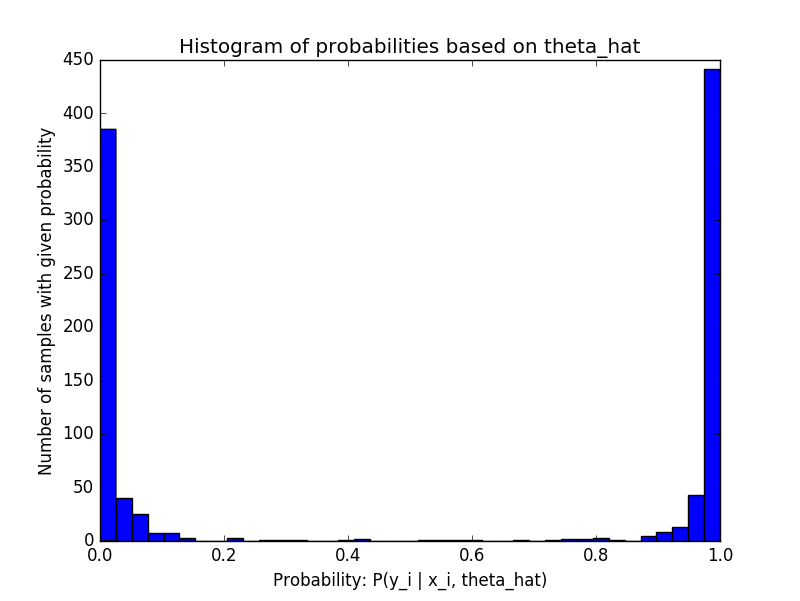
\includegraphics[scale=0.5]{figs/4c_new.png}
  \caption{Histogram of probabilities using Xone.dat and yone.dat}
  \label{fig:4c}
\end{figure}

(d) Figure \ref{fig:4d} shows a histogram plot of the probabilities $P[y_i | x_i;\hat{\theta}]$  based on fitted vector $\hat{\theta}$ and files Xtwo.dat and ytwo.dat.The differences in Figure \ref{fig:4c} and \ref{fig:4d} suggest that it is easier to separate the data in Figure \ref{fig:4c} into two clusters (leading to more accurate fit) than the data in Figure \ref{fig:4d} which is all centered around 0.5.
\begin{figure}[h!]
  \centering
  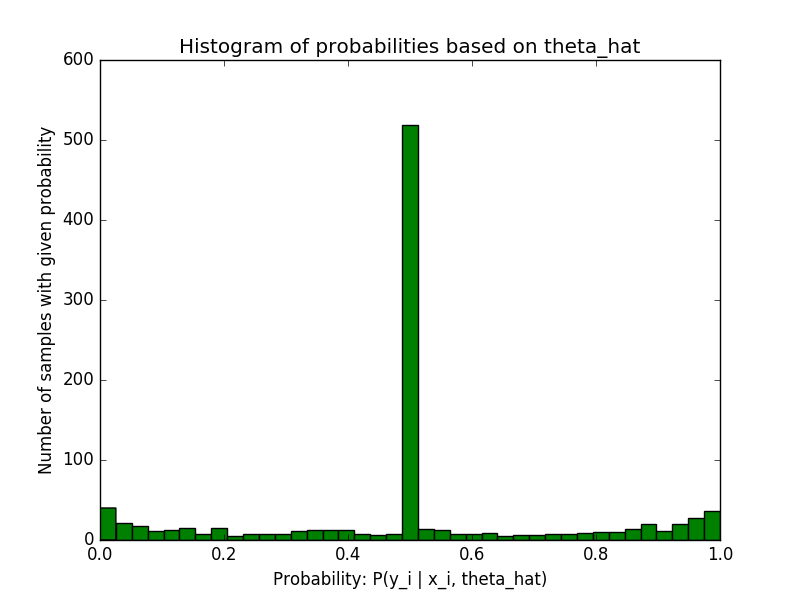
\includegraphics[scale=0.5]{figs/4d.png}
  \caption{Histogram of probabilities using Xtwo.dat and ytwo.dat}
  \label{fig:4d}
\end{figure}

(e) See Figure \ref{fig:4e} for visualization of 2-component GMM to Xone.dat and Xtwo.dat.
\begin{figure}[h!]
  \centering
  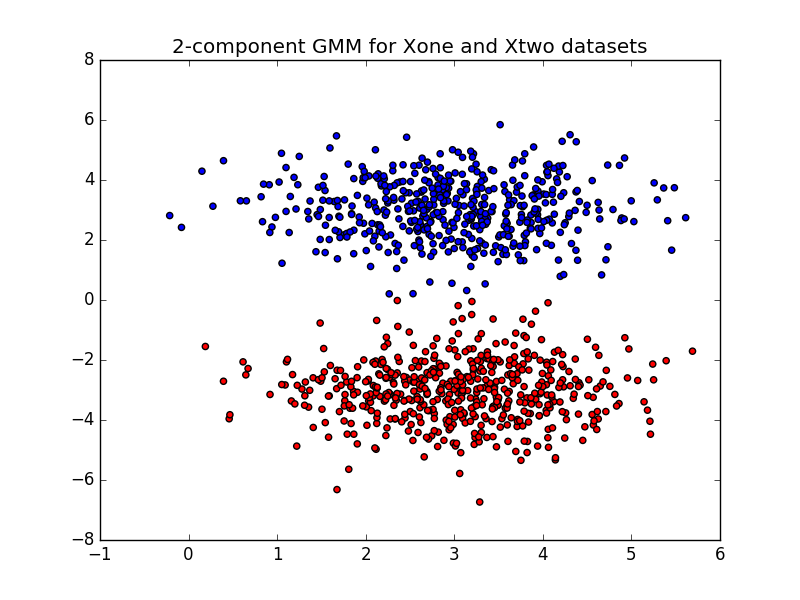
\includegraphics[scale=0.5]{figs/4e.png}
  \caption{Results of fitting a 2-component GMM to Xone.dat and Xtwo.dat}
  \label{fig:4e}
\end{figure}

(f) In part (e), the fitted mean vectors and the $\hat{\theta}$:
\[\mu_{Xone1label}=
	\begin{bmatrix}
		3.03708769\\
		-3.03958106 
	 \end{bmatrix}
   \mu_{Xone0label}=
	\begin{bmatrix}
		2.9674205\\
		3.02468416\\
	 \end{bmatrix}
\]

\[\mu_{Xtwo1label}=
	\begin{bmatrix}
		0.03544899\\
		-0.09377857
	 \end{bmatrix}
   \mu_{Xtwo0label}=
	\begin{bmatrix}
		0.01322437\\
		-0.00039517
	 \end{bmatrix}
\]

\[\hat{\theta}_{LogXone}=
	\begin{bmatrix}
		0.03971547\\
		-1.69052142\\
	 \end{bmatrix}
   \hat{\theta}_{LogXtwo}=
	\begin{bmatrix}
		-0.01176046\\
		-0.02374169\\
	 \end{bmatrix}
\]

\end{problem}

\begin{lstlisting}
'''
Implementation of polynomal fit.
'''

import numpy as np
from numpy import *
import matplotlib.pyplot as plt

# fit a polynomial of degree to t and y data
def polyfit_D(t, y, degree):
	n = len(y)

	# make a [N x (Degree+1)] matrix
	X = np.zeros((n, degree+1))
	for i in range(n):
		for j in range(degree+1):
			X[i][j] = (t[i])**j
	#print X

	# using ordinary least squares
	# compute (X^T*X)^(-1) * X^T * y
	XtX = np.dot(np.transpose(X),X)
	inv_XtX = np.linalg.inv(XtX)
	Xty = np.dot(np.transpose(X),y)
	coeff = np.dot(inv_XtX, Xty)

	return coeff

# returns MSE values for polynomial fitting with degree = [deg_min, deg_max]
# adjusted parameter determines if to add (sigma^2)*DLog(n)/n to MSE value
def polyfit_D_range(t,y,y_tilde,deg_min,deg_max,adjusted):
	i = 0

	MSE_vals = np.zeros(deg_max-deg_min)
	MSE_vals_ytilde = np.zeros(deg_max-deg_min)
	D_vals = np.zeros(deg_max-deg_min)
	# fit the data with a D degree polynomial
	for D in range(deg_min, deg_max):
		# compute coefficients for polynomial of degree D
		coeffs = polyfit_D(t,y,D)
		if(D == 3):
			print coeffs
		# reverse order of coefficients for poly1d function
		rev_coeffs = np.fliplr([coeffs])[0]

		# construct the polynomial for graphing
		polyn = np.poly1d(rev_coeffs)
		# compute mean squared error
		MSE_vals[i] = MSE(t,y,polyn,D)
		MSE_vals_ytilde[i] = MSE(t,y_tilde,polyn,D)
		if(adjusted):
			sigma_2 = 0.25**2
			MSE_vals[i] += (sigma_2*D)*np.log(len(y))/len(y)
		D_vals[i] = D
		i += 1
	return (D_vals, MSE_vals, MSE_vals_ytilde)

# plot MSE vs degree for R(D) and F(D)
def plot_MSE2(D_vals, MSE_vals_y1, MSE_vals_ytilde1):
	# visualize degree vs. MSE
	plt.plot(D_vals, MSE_vals_y1, 'o-b', D_vals, MSE_vals_ytilde1, 'o-g')
	plt.title('Plot of the the mean-squared error vs. degree of polynomial')
	plt.legend(['R(D)', 'R_tilde(D)'])
	plt.xlabel('D values')
	plt.ylabel('Mean-squared error')
	plt.show()

# compute mean squared error for estimated polynomial of degree D
def MSE(t, y, polyn, D):
	n = len(y)
	sum = 0.0
	for i in range(0,n):
		sum += (y[i] - polyn(t[i])) ** 2

	return sum/n

if __name__ == "__main__":
	t = np.loadtxt('data_problem2.1/t.dat')
	y_orig = np.loadtxt('data_problem2.1/y.dat')
	y_fresh = np.loadtxt('data_problem2.1/yfresh.dat')

	# choose a y data source
	y = y_orig
	n = len(y) # 9 in this case

	# R(D), R_tilde(D)
	(D_vals1, MSE_vals_y1, MSE_vals_ytilde1) = polyfit_D_range(t, y_orig, y_fresh, 2, 10, 0);
	# F(D), F_tilde(D)
	(D_vals2, MSE_vals_y2, MSE_vals_ytilde2) = polyfit_D_range(t, y_orig, y_fresh, 2, 10, 1);

	plot_MSE2(D_vals1, MSE_vals_y1, MSE_vals_ytilde1)
	plot_MSE2(D_vals2, MSE_vals_ytilde1, MSE_vals_y2)

\end{lstlisting}

\begin{lstlisting}
"""
Implementation of stochastic gradient descent.
"""
import numpy as np
from numpy import *
import matplotlib.pyplot as plt

def log_loss(X,y,theta):
    sum = 0
    for i in range(m):
        sum += log(1+np.exp(-y[i]*((theta.T)*X[i] + b)))
    sum = -sum

def stoch_gd(X, y, numIter, stepSize, epsilon):
    (m,n) = np.shape(X)
    theta = np.random.rand(n)

    # begin iterations
    for i in range(numIter):
        I = np.random.randint(0,m)

        # extheta = np.exp((theta.T)*X[I])
        # compute the gradient at the current location
        g = y[I]*X[I] - X[I]*1.0/(1.0+np.exp(-(theta.T)*X[I]))

        # step in the direction of the gradient
        theta2 = theta + (1.0/(i+1.0))*g

        if(np.dot(theta2-theta, theta2-theta) < epsilon):
            return theta
        else:
            theta = theta2

    # return the solution
    return theta


if __name__ == '__main__':
    Xone = np.loadtxt('data_problem2.4/Xone.dat')
    yone = np.loadtxt('data_problem2.4/yone.dat')

    Xtwo = np.loadtxt('data_problem2.4/Xtwo.dat')
    ytwo = np.loadtxt('data_problem2.4/ytwo.dat')

    (m,n) = np.shape(Xone)
    # take number of iterations to be number of examples
    numIter = 10000
    epsilon = 0.0000000000001
    stepSize = 0.01

    # data set #1
    theta_hat1 = stoch_gd(Xone, yone, numIter, stepSize, epsilon)
    e_yxtheta1 = np.exp(-np.dot(Xone,theta_hat1))
    p_one = 1.0/(1.0+e_yxtheta1)

    # data set #2
    theta_hat2 = stoch_gd(Xtwo, ytwo, numIter, stepSize, epsilon)
    e_yxtheta2 = np.exp(-np.dot(Xtwo,theta_hat2))
    p_two = 1.0/(1.0+e_yxtheta2)

    print theta_hat1
    print theta_hat2

    bins = np.linspace(0, 1, 40)

    plt.title("Histogram of probabilities based on theta_hat")
    plt.xlabel("Probability: P(y_i | x_i, theta_hat)")
    plt.ylabel("Number of samples with given probability")
    #plt.hist(p_one, bins)
    plt.hist(p_two, bins, facecolor='green')
    plt.show()
\end{lstlisting}

\begin{lstlisting}
"""
Implementation of 2-component GMM.
"""
import numpy as np
from numpy import *
import matplotlib.pyplot as plt
from sklearn import mixture

def run_gmm(X, num_components):
    gmm = mixture.GMM(n_components=num_components, covariance_type='full')
    gmm.fit(X)
    print gmm.means_
    colors = ['r' if i==0 else 'b' for i in gmm.predict(X)]
    p = plt.gca()
    p.scatter(X[:,0], X[:,1], c=colors)
    plt.title("2-component GMM for Xone and Xtwo datasets")
    plt.show()


if __name__ == '__main__':
    Xone = np.loadtxt('data_problem2.4/Xone.dat')
    Xtwo = np.loadtxt('data_problem2.4/Xtwo.dat')

    yone = np.loadtxt('data_problem2.4/yone.dat')
    ytwo = np.loadtxt('data_problem2.4/ytwo.dat')

    X = np.concatenate((Xone, Xtwo), axis=1)

    run_gmm(X, 2)
\end{lstlisting}
\end{document}